\section{LIME}

LIME \cite{ribeiro2016should} is a black box interpretability method. Like all black box methods, LIME randomly changes features in the input data to detect which feature is relevant for a specific classification.

In the case of image classification, LIME does not modify single pixels, because this would generate too many different versions of the input.
Instead, LIME generates superpixels.

\begin{figure}[H]
    \centering
    \begin{subfigure}[t]{.35\textwidth}
        \centering
        
\includegraphics[width=\linewidth]{chapters/02_methods/images/frog1.png}
        \caption{Original image}
    \end{subfigure}\hspace{1.5cm}%
    \begin{subfigure}[t]{.35\textwidth}
        \centering
        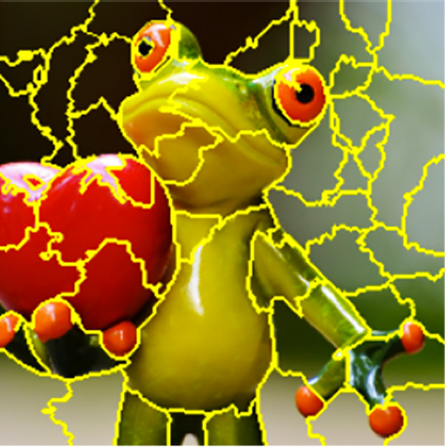
\includegraphics[width=\linewidth]{chapters/02_methods/images/frog2.png}
        \caption{Original image overlaid with superpixel boundaries}
    \end{subfigure}
    \caption{Superpixels generated for an input image. Superpixels are the features LIME analyzes to detect if they are relevant for the classification.\cite{limeoreilly}}
    \label{lime_superpixel}
\end{figure}


Superpixels are continuous regions on an image with a similar color. In the Python reference implementation, LIME uses the Quick Shift \cite{vedaldi2008quick} clustering algorithm to generate these superpixels. Figure \ref{lime_superpixel} shows superpixels overlaid on an example image.

\begin{figure}[H]
\centering
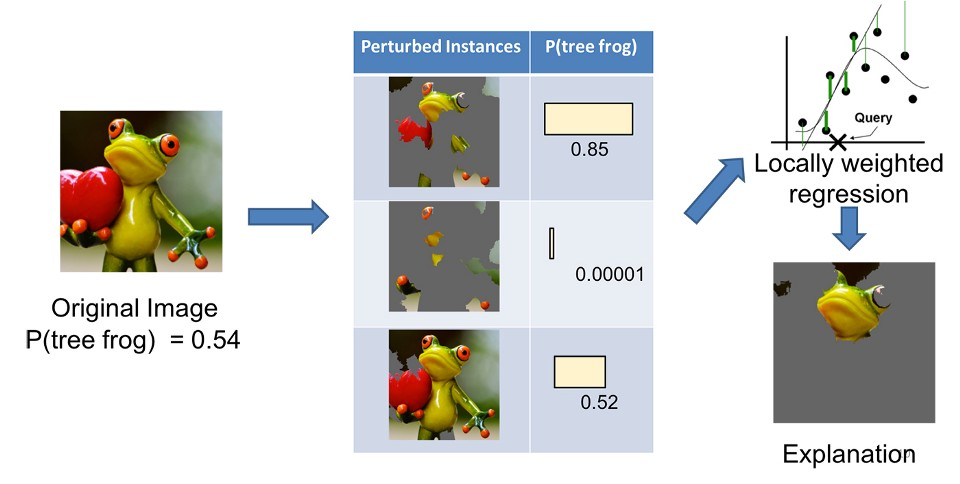
\includegraphics[width=14cm]{chapters/02_methods/images/lime2.jpg}
\caption{Left: Original image with detected class and probability. Center: Perturbed images generated by randomly turning off superpixels and their probability for the specific class.
Right: Locally weighted regression to generate a preferably continuous region to explain the class.\cite{limeoreilly}}
\label{lime_perturbed}
\end{figure}

In the next step, LIME generates input images by turning off multiple randomly selected superpixels. Turning off in this case means setting the color inside the superpixel to gray. The center image of Figure \ref{lime_perturbed} shows some examples of deactivated superpixels. The generated input images are then run trough the neural network and the changed probabilities of the relevant class(es) are recorded. As a last step, LIME does a locally weighted (i.e. adjacent superpixels are weighted higher) regression of the probabilities to generate a preferably continuous cluster of superpixels explaining a specific class (right image in Figure \ref{lime_perturbed}).

For visualization, the original image is taken and all pixels that are outside of the superpixel cluster deemed relevant for the classification are grayed out.
Figure \ref{lime_dog} shows a visualization for three classes on a complex input image. Alternativly, the superpixel cluster is drawn over the input image with transparency.

\begin{figure}[H]
    \centering
    \begin{subfigure}[t]{.23\textwidth}
        \centering
        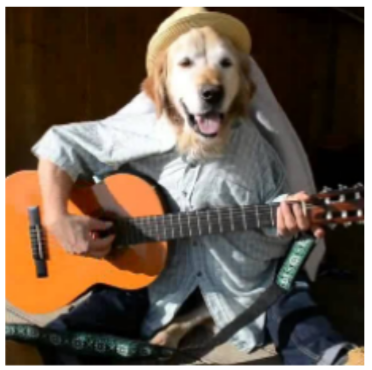
\includegraphics[width=\linewidth]{chapters/02_methods/images/lime_dog_1.png}
        \caption{Original image}
    \end{subfigure}\hfill%
    \begin{subfigure}[t]{.23\textwidth}
        \centering
        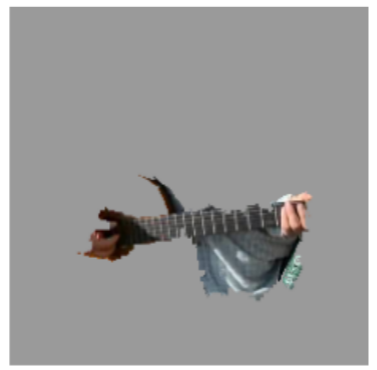
\includegraphics[width=\linewidth]{chapters/02_methods/images/lime_dog_2.png}
        \caption{Explain class Electric guitar (p=0.32)}
    \end{subfigure}\hfill%
    \begin{subfigure}[t]{.23\textwidth}
        \centering
        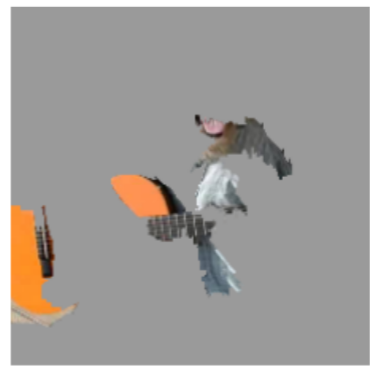
\includegraphics[width=\linewidth]{chapters/02_methods/images/lime_dog_3.png}
        \caption{Explain class Acoustic guitar (p=0.24}
    \end{subfigure}\hfill%
    \begin{subfigure}[t]{.23\textwidth}
        \centering
        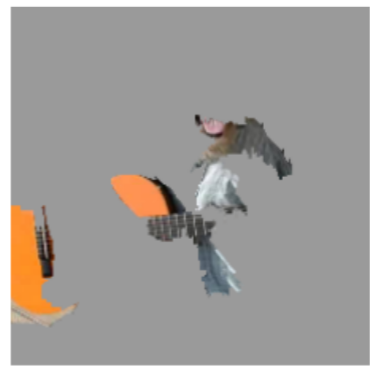
\includegraphics[width=\linewidth]{chapters/02_methods/images/lime_dog_3.png}
        \caption{Explain class Labrador (p=0.21}
    \end{subfigure}
    \caption{Explaining the top 3 classes on an example image with LIME. The used neural network architecture is Inception trained on ImageNet.\cite{ribeiro2016should}}
    \label{lime_dog}
\end{figure}
